\documentclass[1p]{elsarticle_modified}
%\bibliographystyle{elsarticle-num}

%\usepackage[colorlinks]{hyperref}
%\usepackage{abbrmath_seonhwa} %\Abb, \Ascr, \Acal ,\Abf, \Afrak
\usepackage{amsfonts}
\usepackage{amssymb}
\usepackage{amsmath}
\usepackage{amsthm}
\usepackage{scalefnt}
\usepackage{amsbsy}
\usepackage{kotex}
\usepackage{caption}
\usepackage{subfig}
\usepackage{color}
\usepackage{graphicx}
\usepackage{xcolor} %% white, black, red, green, blue, cyan, magenta, yellow
\usepackage{float}
\usepackage{setspace}
\usepackage{hyperref}

\usepackage{tikz}
\usetikzlibrary{arrows}

\usepackage{multirow}
\usepackage{array} % fixed length table
\usepackage{hhline}

%%%%%%%%%%%%%%%%%%%%%
\makeatletter
\renewcommand*\env@matrix[1][\arraystretch]{%
	\edef\arraystretch{#1}%
	\hskip -\arraycolsep
	\let\@ifnextchar\new@ifnextchar
	\array{*\c@MaxMatrixCols c}}
\makeatother %https://tex.stackexchange.com/questions/14071/how-can-i-increase-the-line-spacing-in-a-matrix
%%%%%%%%%%%%%%%

\usepackage[normalem]{ulem}

\newcommand{\msout}[1]{\ifmmode\text{\sout{\ensuremath{#1}}}\else\sout{#1}\fi}
%SOURCE: \msout is \stkout macro in https://tex.stackexchange.com/questions/20609/strikeout-in-math-mode

\newcommand{\cancel}[1]{
	\ifmmode
	{\color{red}\msout{#1}}
	\else
	{\color{red}\sout{#1}}
	\fi
}

\newcommand{\add}[1]{
	{\color{blue}\uwave{#1}}
}

\newcommand{\replace}[2]{
	\ifmmode
	{\color{red}\msout{#1}}{\color{blue}\uwave{#2}}
	\else
	{\color{red}\sout{#1}}{\color{blue}\uwave{#2}}
	\fi
}

\newcommand{\Sol}{\mathcal{S}} %segment
\newcommand{\D}{D} %diagram
\newcommand{\A}{\mathcal{A}} %arc


%%%%%%%%%%%%%%%%%%%%%%%%%%%%%5 test

\def\sl{\operatorname{\textup{SL}}(2,\Cbb)}
\def\psl{\operatorname{\textup{PSL}}(2,\Cbb)}
\def\quan{\mkern 1mu \triangleright \mkern 1mu}

\theoremstyle{definition}
\newtheorem{thm}{Theorem}[section]
\newtheorem{prop}[thm]{Proposition}
\newtheorem{lem}[thm]{Lemma}
\newtheorem{ques}[thm]{Question}
\newtheorem{cor}[thm]{Corollary}
\newtheorem{defn}[thm]{Definition}
\newtheorem{exam}[thm]{Example}
\newtheorem{rmk}[thm]{Remark}
\newtheorem{alg}[thm]{Algorithm}

\newcommand{\I}{\sqrt{-1}}
\begin{document}

%\begin{frontmatter}
%
%\title{Boundary parabolic representations of knots up to 8 crossings}
%
%%% Group authors per affiliation:
%\author{Yunhi Cho} 
%\address{Department of Mathematics, University of Seoul, Seoul, Korea}
%\ead{yhcho@uos.ac.kr}
%
%
%\author{Seonhwa Kim} %\fnref{s_kim}}
%\address{Center for Geometry and Physics, Institute for Basic Science, Pohang, 37673, Korea}
%\ead{ryeona17@ibs.re.kr}
%
%\author{Hyuk Kim}
%\address{Department of Mathematical Sciences, Seoul National University, Seoul 08826, Korea}
%\ead{hyukkim@snu.ac.kr}
%
%\author{Seokbeom Yoon}
%\address{Department of Mathematical Sciences, Seoul National University, Seoul, 08826,  Korea}
%\ead{sbyoon15@snu.ac.kr}
%
%\begin{abstract}
%We find all boundary parabolic representation of knots up to 8 crossings.
%
%\end{abstract}
%\begin{keyword}
%    \MSC[2010] 57M25 
%\end{keyword}
%
%\end{frontmatter}

%\linenumbers
%\tableofcontents
%
\newcommand\colored[1]{\textcolor{white}{\rule[-0.35ex]{0.8em}{1.4ex}}\kern-0.8em\color{red} #1}%
%\newcommand\colored[1]{\textcolor{white}{ #1}\kern-2.17ex	\textcolor{white}{ #1}\kern-1.81ex	\textcolor{white}{ #1}\kern-2.15ex\color{red}#1	}

{\Large $\underline{12a_{0410}~(K12a_{0410})}$}

\setlength{\tabcolsep}{10pt}
\renewcommand{\arraystretch}{1.6}
\vspace{1cm}\begin{tabular}{m{100pt}>{\centering\arraybackslash}m{274pt}}
\multirow{5}{120pt}{
	\centering
	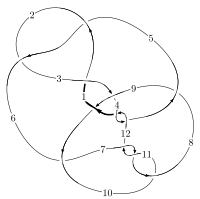
\includegraphics[width=112pt]{../../../GIT/diagram.site/Diagrams/png/1211_12a_0410.png}\\
\ \ \ A knot diagram\footnotemark}&
\allowdisplaybreaks
\textbf{Linearized knot diagam} \\
\cline{2-2}
 &
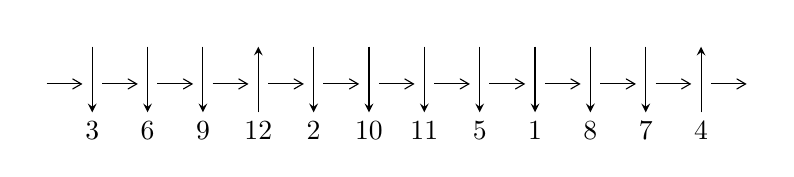
\begin{tikzpicture}[x=20pt, y=17pt]
	% nodes
	\node (C0) at (0, 0) {};
	\node (C1) at (1, 0) {};
	\node (C1U) at (1, +1) {};
	\node (C1D) at (1, -1) {3};

	\node (C2) at (2, 0) {};
	\node (C2U) at (2, +1) {};
	\node (C2D) at (2, -1) {6};

	\node (C3) at (3, 0) {};
	\node (C3U) at (3, +1) {};
	\node (C3D) at (3, -1) {9};

	\node (C4) at (4, 0) {};
	\node (C4U) at (4, +1) {};
	\node (C4D) at (4, -1) {12};

	\node (C5) at (5, 0) {};
	\node (C5U) at (5, +1) {};
	\node (C5D) at (5, -1) {2};

	\node (C6) at (6, 0) {};
	\node (C6U) at (6, +1) {};
	\node (C6D) at (6, -1) {10};

	\node (C7) at (7, 0) {};
	\node (C7U) at (7, +1) {};
	\node (C7D) at (7, -1) {11};

	\node (C8) at (8, 0) {};
	\node (C8U) at (8, +1) {};
	\node (C8D) at (8, -1) {5};

	\node (C9) at (9, 0) {};
	\node (C9U) at (9, +1) {};
	\node (C9D) at (9, -1) {1};

	\node (C10) at (10, 0) {};
	\node (C10U) at (10, +1) {};
	\node (C10D) at (10, -1) {8};

	\node (C11) at (11, 0) {};
	\node (C11U) at (11, +1) {};
	\node (C11D) at (11, -1) {7};

	\node (C12) at (12, 0) {};
	\node (C12U) at (12, +1) {};
	\node (C12D) at (12, -1) {4};
	\node (C13) at (13, 0) {};

	% arrows
	\draw[->,>={angle 60}]
	(C0) edge (C1) (C1) edge (C2) (C2) edge (C3) (C3) edge (C4) (C4) edge (C5) (C5) edge (C6) (C6) edge (C7) (C7) edge (C8) (C8) edge (C9) (C9) edge (C10) (C10) edge (C11) (C11) edge (C12) (C12) edge (C13) ;	\draw[->,>=stealth]
	(C1U) edge (C1D) (C2U) edge (C2D) (C3U) edge (C3D) (C4D) edge (C4U) (C5U) edge (C5D) (C6U) edge (C6D) (C7U) edge (C7D) (C8U) edge (C8D) (C9U) edge (C9D) (C10U) edge (C10D) (C11U) edge (C11D) (C12D) edge (C12U) ;
	\end{tikzpicture} \\
\hhline{~~} \\& 
\textbf{Solving Sequence} \\ \cline{2-2} 
 &
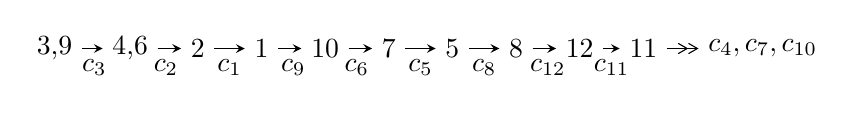
\begin{tikzpicture}[x=23pt, y=7pt]
	% node
	\node (A0) at (-1/8, 0) {3,9};
	\node (A1) at (17/16, 0) {4,6};
	\node (A2) at (17/8, 0) {2};
	\node (A3) at (25/8, 0) {1};
	\node (A4) at (33/8, 0) {10};
	\node (A5) at (41/8, 0) {7};
	\node (A6) at (49/8, 0) {5};
	\node (A7) at (57/8, 0) {8};
	\node (A8) at (65/8, 0) {12};
	\node (A9) at (73/8, 0) {11};
	\node (C1) at (1/2, -1) {$c_{3}$};
	\node (C2) at (13/8, -1) {$c_{2}$};
	\node (C3) at (21/8, -1) {$c_{1}$};
	\node (C4) at (29/8, -1) {$c_{9}$};
	\node (C5) at (37/8, -1) {$c_{6}$};
	\node (C6) at (45/8, -1) {$c_{5}$};
	\node (C7) at (53/8, -1) {$c_{8}$};
	\node (C8) at (61/8, -1) {$c_{12}$};
	\node (C9) at (69/8, -1) {$c_{11}$};
	\node (A10) at (11, 0) {$c_{4},c_{7},c_{10}$};

	% edge
	\draw[->,>=stealth]	
	(A0) edge (A1) (A1) edge (A2) (A2) edge (A3) (A3) edge (A4) (A4) edge (A5) (A5) edge (A6) (A6) edge (A7) (A7) edge (A8) (A8) edge (A9) ;
	\draw[->>,>={angle 60}]	
	(A9) edge (A10);
\end{tikzpicture} \\ 

\end{tabular} \\

\footnotetext{
The image of knot diagram is generated by the software ``\textbf{Draw programme}" developed by Andrew Bartholomew(\url{http://www.layer8.co.uk/maths/draw/index.htm\#Running-draw}), where we modified some parts for our purpose(\url{https://github.com/CATsTAILs/LinksPainter}).
}\phantom \\ \newline 
\centering \textbf{Ideals for irreducible components\footnotemark of $X_{\text{par}}$} 
 
\begin{align*}
I^u_{1}&=\langle 
4.25183\times10^{585} u^{103}-3.49672\times10^{585} u^{102}+\cdots+8.74093\times10^{585} b+3.71015\times10^{586},\\
\phantom{I^u_{1}}&\phantom{= \langle  }6.16669\times10^{587} u^{103}-4.95476\times10^{587} u^{102}+\cdots+8.74093\times10^{585} a+3.40901\times10^{588},\;u^{104}- u^{103}+\cdots+4 u-1\rangle \\
\\
\end{align*}
\raggedright * 1 irreducible components of $\dim_{\mathbb{C}}=0$, with total 104 representations.\\
\footnotetext{All coefficients of polynomials are rational numbers. But the coefficients are sometimes approximated in decimal forms when there is not enough margin.}
\newpage
\renewcommand{\arraystretch}{1}
\centering \section*{I. $I^u_{1}= \langle 4.25\times10^{585} u^{103}-3.50\times10^{585} u^{102}+\cdots+8.74\times10^{585} b+3.71\times10^{586},\;6.17\times10^{587} u^{103}-4.95\times10^{587} u^{102}+\cdots+8.74\times10^{585} a+3.41\times10^{588},\;u^{104}- u^{103}+\cdots+4 u-1 \rangle$}
\flushleft \textbf{(i) Arc colorings}\\
\begin{tabular}{m{7pt} m{180pt} m{7pt} m{180pt} }
\flushright $a_{3}=$&$\begin{pmatrix}1\\0\end{pmatrix}$ \\
\flushright $a_{9}=$&$\begin{pmatrix}0\\u\end{pmatrix}$ \\
\flushright $a_{4}=$&$\begin{pmatrix}1\\u^2\end{pmatrix}$ \\
\flushright $a_{6}=$&$\begin{pmatrix}-70.5495 u^{103}+56.6846 u^{102}+\cdots-557.720 u-390.005\\-0.486427 u^{103}+0.400040 u^{102}+\cdots-5.53020 u-4.24457\end{pmatrix}$ \\
\flushright $a_{2}=$&$\begin{pmatrix}-102.717 u^{103}+81.0025 u^{102}+\cdots-543.733 u-496.837\\-1.37667 u^{103}+1.15211 u^{102}+\cdots-9.54433 u-8.96963\end{pmatrix}$ \\
\flushright $a_{1}=$&$\begin{pmatrix}-104.094 u^{103}+82.1546 u^{102}+\cdots-553.277 u-505.807\\-1.37667 u^{103}+1.15211 u^{102}+\cdots-9.54433 u-8.96963\end{pmatrix}$ \\
\flushright $a_{10}=$&$\begin{pmatrix}-323.391 u^{103}+228.074 u^{102}+\cdots+978.592 u-1309.82\\-15.2283 u^{103}+12.0817 u^{102}+\cdots+0.583226 u-70.8551\end{pmatrix}$ \\
\flushright $a_{7}=$&$\begin{pmatrix}203.528 u^{103}-157.623 u^{102}+\cdots-787.570 u+388.116\\9.83386 u^{103}-7.22442 u^{102}+\cdots+26.3806 u+44.1586\end{pmatrix}$ \\
\flushright $a_{5}=$&$\begin{pmatrix}24.0836 u^{103}-18.0365 u^{102}+\cdots-147.484 u+38.3478\\2.09265 u^{103}-1.51733 u^{102}+\cdots+0.457127 u+8.25296\end{pmatrix}$ \\
\flushright $a_{8}=$&$\begin{pmatrix}-250.120 u^{103}+167.113 u^{102}+\cdots+1343.51 u-959.073\\-14.4955 u^{103}+11.4521 u^{102}+\cdots+12.7671 u-66.7521\end{pmatrix}$ \\
\flushright $a_{12}=$&$\begin{pmatrix}-106.712 u^{103}+84.1220 u^{102}+\cdots-560.070 u-518.776\\-1.53073 u^{103}+1.27128 u^{102}+\cdots-9.55960 u-9.62036\end{pmatrix}$ \\
\flushright $a_{11}=$&$\begin{pmatrix}-195.042 u^{103}+137.460 u^{102}+\cdots-980.891 u-659.152\\-5.95727 u^{103}+4.33298 u^{102}+\cdots+14.3247 u-39.1433\end{pmatrix}$\\&\end{tabular}
\flushleft \textbf{(ii) Obstruction class $= -1$}\\~\\
\flushleft \textbf{(iii) Cusp Shapes $= 8.88084 u^{103}-5.44978 u^{102}+\cdots-468.605 u-98.2415$}\\~\\
\newpage\renewcommand{\arraystretch}{1}
\flushleft \textbf{(iv) u-Polynomials at the component}\newline \\
\begin{tabular}{m{50pt}|m{274pt}}
Crossings & \hspace{64pt}u-Polynomials at each crossing \\
\hline $$\begin{aligned}c_{1}\end{aligned}$$&$\begin{aligned}
&u^{104}+43 u^{103}+\cdots+20 u+1
\end{aligned}$\\
\hline $$\begin{aligned}c_{2},c_{5}\end{aligned}$$&$\begin{aligned}
&u^{104}+7 u^{103}+\cdots+6 u+1
\end{aligned}$\\
\hline $$\begin{aligned}c_{3}\end{aligned}$$&$\begin{aligned}
&u^{104}- u^{103}+\cdots+4 u-1
\end{aligned}$\\
\hline $$\begin{aligned}c_{4},c_{12}\end{aligned}$$&$\begin{aligned}
&u^{104}+7 u^{103}+\cdots+6 u+1
\end{aligned}$\\
\hline $$\begin{aligned}c_{6}\end{aligned}$$&$\begin{aligned}
&u^{104}+u^{103}+\cdots-159742 u-10001
\end{aligned}$\\
\hline $$\begin{aligned}c_{7},c_{10},c_{11}\end{aligned}$$&$\begin{aligned}
&u^{104}- u^{103}+\cdots-16 u-1
\end{aligned}$\\
\hline $$\begin{aligned}c_{8}\end{aligned}$$&$\begin{aligned}
&u^{104}+5 u^{103}+\cdots+1611520 u-285184
\end{aligned}$\\
\hline $$\begin{aligned}c_{9}\end{aligned}$$&$\begin{aligned}
&u^{104}+7 u^{103}+\cdots+14816 u+928
\end{aligned}$\\
\hline
\end{tabular}\\~\\
\newpage\renewcommand{\arraystretch}{1}
\flushleft \textbf{(v) Riley Polynomials at the component}\newline \\
\begin{tabular}{m{50pt}|m{274pt}}
Crossings & \hspace{64pt}Riley Polynomials at each crossing \\
\hline $$\begin{aligned}c_{1}\end{aligned}$$&$\begin{aligned}
&y^{104}+37 y^{103}+\cdots-404 y+1
\end{aligned}$\\
\hline $$\begin{aligned}c_{2},c_{5}\end{aligned}$$&$\begin{aligned}
&y^{104}-43 y^{103}+\cdots-20 y+1
\end{aligned}$\\
\hline $$\begin{aligned}c_{3}\end{aligned}$$&$\begin{aligned}
&y^{104}-7 y^{103}+\cdots-84 y+1
\end{aligned}$\\
\hline $$\begin{aligned}c_{4},c_{12}\end{aligned}$$&$\begin{aligned}
&y^{104}+73 y^{103}+\cdots-20 y+1
\end{aligned}$\\
\hline $$\begin{aligned}c_{6}\end{aligned}$$&$\begin{aligned}
&y^{104}-35 y^{103}+\cdots-15905585468 y+100020001
\end{aligned}$\\
\hline $$\begin{aligned}c_{7},c_{10},c_{11}\end{aligned}$$&$\begin{aligned}
&y^{104}+89 y^{103}+\cdots-156 y+1
\end{aligned}$\\
\hline $$\begin{aligned}c_{8}\end{aligned}$$&$\begin{aligned}
&y^{104}-199 y^{103}+\cdots-3752188116992 y+81329913856
\end{aligned}$\\
\hline $$\begin{aligned}c_{9}\end{aligned}$$&$\begin{aligned}
&y^{104}+145 y^{103}+\cdots-51493888 y+861184
\end{aligned}$\\
\hline
\end{tabular}\\~\\
\newpage\flushleft \textbf{(vi) Complex Volumes and Cusp Shapes}
$$\begin{array}{c|c|c}  
\text{Solutions to }I^u_{1}& \I (\text{vol} + \sqrt{-1}CS) & \text{Cusp shape}\\
 \hline 
\begin{aligned}
u &= \phantom{-}0.563363 + 0.821946 I \\
a &= \phantom{-}0.444185 - 0.891149 I \\
b &= -0.454391 + 0.989162 I\end{aligned}
 & \phantom{-}6.57214 - 6.48719 I & \phantom{-0.000000 } 0 \\ \hline\begin{aligned}
u &= \phantom{-}0.563363 - 0.821946 I \\
a &= \phantom{-}0.444185 + 0.891149 I \\
b &= -0.454391 - 0.989162 I\end{aligned}
 & \phantom{-}6.57214 + 6.48719 I & \phantom{-0.000000 } 0 \\ \hline\begin{aligned}
u &= -0.621126 + 0.769884 I \\
a &= -0.56396 - 1.81731 I \\
b &= -1.029360 + 0.485493 I\end{aligned}
 & \phantom{-}1.01084 + 5.03860 I & \phantom{-0.000000 } 0 \\ \hline\begin{aligned}
u &= -0.621126 - 0.769884 I \\
a &= -0.56396 + 1.81731 I \\
b &= -1.029360 - 0.485493 I\end{aligned}
 & \phantom{-}1.01084 - 5.03860 I & \phantom{-0.000000 } 0 \\ \hline\begin{aligned}
u &= \phantom{-}0.388922 + 0.904890 I \\
a &= \phantom{-}0.596870 - 0.870016 I \\
b &= -0.542166 + 0.717661 I\end{aligned}
 & \phantom{-}2.80919 + 0.07810 I & \phantom{-0.000000 } 0 \\ \hline\begin{aligned}
u &= \phantom{-}0.388922 - 0.904890 I \\
a &= \phantom{-}0.596870 + 0.870016 I \\
b &= -0.542166 - 0.717661 I\end{aligned}
 & \phantom{-}2.80919 - 0.07810 I & \phantom{-0.000000 } 0 \\ \hline\begin{aligned}
u &= \phantom{-}0.970515 + 0.147136 I \\
a &= \phantom{-}0.875999 - 0.444927 I \\
b &= \phantom{-}0.674437 + 0.541246 I\end{aligned}
 & \phantom{-}4.46398 + 2.11638 I & \phantom{-0.000000 } 0 \\ \hline\begin{aligned}
u &= \phantom{-}0.970515 - 0.147136 I \\
a &= \phantom{-}0.875999 + 0.444927 I \\
b &= \phantom{-}0.674437 - 0.541246 I\end{aligned}
 & \phantom{-}4.46398 - 2.11638 I & \phantom{-0.000000 } 0 \\ \hline\begin{aligned}
u &= -0.505334 + 0.804558 I \\
a &= \phantom{-}0.453957 + 0.831515 I \\
b &= -0.399937 - 0.890019 I\end{aligned}
 & \phantom{-}1.50309 + 3.13338 I & \phantom{-0.000000 } 0 \\ \hline\begin{aligned}
u &= -0.505334 - 0.804558 I \\
a &= \phantom{-}0.453957 - 0.831515 I \\
b &= -0.399937 + 0.890019 I\end{aligned}
 & \phantom{-}1.50309 - 3.13338 I & \phantom{-0.000000 } 0\\
 \hline 
 \end{array}$$\newpage$$\begin{array}{c|c|c}  
\text{Solutions to }I^u_{1}& \I (\text{vol} + \sqrt{-1}CS) & \text{Cusp shape}\\
 \hline 
\begin{aligned}
u &= \phantom{-}0.825078 + 0.437544 I \\
a &= \phantom{-}0.366274 - 0.209695 I \\
b &= \phantom{-}0.946141 - 0.486683 I\end{aligned}
 & -1.62694 + 3.28109 I & \phantom{-0.000000 } 0 \\ \hline\begin{aligned}
u &= \phantom{-}0.825078 - 0.437544 I \\
a &= \phantom{-}0.366274 + 0.209695 I \\
b &= \phantom{-}0.946141 + 0.486683 I\end{aligned}
 & -1.62694 - 3.28109 I & \phantom{-0.000000 } 0 \\ \hline\begin{aligned}
u &= -0.960850 + 0.560302 I \\
a &= \phantom{-}0.0740763 + 0.0415182 I \\
b &= \phantom{-}0.959373 + 0.560649 I\end{aligned}
 & \phantom{-}3.58609 - 6.59895 I & \phantom{-0.000000 } 0 \\ \hline\begin{aligned}
u &= -0.960850 - 0.560302 I \\
a &= \phantom{-}0.0740763 - 0.0415182 I \\
b &= \phantom{-}0.959373 - 0.560649 I\end{aligned}
 & \phantom{-}3.58609 + 6.59895 I & \phantom{-0.000000 } 0 \\ \hline\begin{aligned}
u &= -0.808529 + 0.272807 I \\
a &= -0.32342 - 2.08395 I \\
b &= -0.530241 - 0.185700 I\end{aligned}
 & \phantom{-}1.61075 - 4.42335 I & \phantom{-0.000000 } 0 \\ \hline\begin{aligned}
u &= -0.808529 - 0.272807 I \\
a &= -0.32342 + 2.08395 I \\
b &= -0.530241 + 0.185700 I\end{aligned}
 & \phantom{-}1.61075 + 4.42335 I & \phantom{-0.000000 } 0 \\ \hline\begin{aligned}
u &= -0.717693 + 0.898837 I \\
a &= -0.28560 - 1.56028 I \\
b &= -1.060130 + 0.592917 I\end{aligned}
 & \phantom{-}1.24152 + 4.96360 I & \phantom{-0.000000 } 0 \\ \hline\begin{aligned}
u &= -0.717693 - 0.898837 I \\
a &= -0.28560 + 1.56028 I \\
b &= -1.060130 - 0.592917 I\end{aligned}
 & \phantom{-}1.24152 - 4.96360 I & \phantom{-0.000000 } 0 \\ \hline\begin{aligned}
u &= -0.520163 + 1.029420 I \\
a &= \phantom{-}0.516539 + 0.934515 I \\
b &= -0.693321 - 0.824652 I\end{aligned}
 & \phantom{-}8.89831 - 1.49693 I & \phantom{-0.000000 } 0 \\ \hline\begin{aligned}
u &= -0.520163 - 1.029420 I \\
a &= \phantom{-}0.516539 - 0.934515 I \\
b &= -0.693321 + 0.824652 I\end{aligned}
 & \phantom{-}8.89831 + 1.49693 I & \phantom{-0.000000 } 0\\
 \hline 
 \end{array}$$\newpage$$\begin{array}{c|c|c}  
\text{Solutions to }I^u_{1}& \I (\text{vol} + \sqrt{-1}CS) & \text{Cusp shape}\\
 \hline 
\begin{aligned}
u &= \phantom{-}0.241022 + 0.772602 I \\
a &= \phantom{-}0.79562 + 2.59697 I \\
b &= -0.901827 - 0.433942 I\end{aligned}
 & -2.08746 - 1.73740 I & \phantom{-0.000000 } 0 \\ \hline\begin{aligned}
u &= \phantom{-}0.241022 - 0.772602 I \\
a &= \phantom{-}0.79562 - 2.59697 I \\
b &= -0.901827 + 0.433942 I\end{aligned}
 & -2.08746 + 1.73740 I & \phantom{-0.000000 } 0 \\ \hline\begin{aligned}
u &= \phantom{-}0.803988 + 0.896157 I \\
a &= -0.25183 + 1.43561 I \\
b &= -1.138880 - 0.645059 I\end{aligned}
 & -0.70178 - 8.77355 I & \phantom{-0.000000 } 0 \\ \hline\begin{aligned}
u &= \phantom{-}0.803988 - 0.896157 I \\
a &= -0.25183 - 1.43561 I \\
b &= -1.138880 + 0.645059 I\end{aligned}
 & -0.70178 + 8.77355 I & \phantom{-0.000000 } 0 \\ \hline\begin{aligned}
u &= \phantom{-}0.497385 + 0.621008 I \\
a &= \phantom{-}0.078179 - 0.664644 I \\
b &= \phantom{-}0.056824 + 0.865095 I\end{aligned}
 & \phantom{-}4.05431 - 1.11668 I & \phantom{-0.000000 } 0 \\ \hline\begin{aligned}
u &= \phantom{-}0.497385 - 0.621008 I \\
a &= \phantom{-}0.078179 + 0.664644 I \\
b &= \phantom{-}0.056824 - 0.865095 I\end{aligned}
 & \phantom{-}4.05431 + 1.11668 I & \phantom{-0.000000 } 0 \\ \hline\begin{aligned}
u &= -0.791300 + 0.046534 I \\
a &= \phantom{-}0.815917 - 0.154042 I \\
b &= \phantom{-}0.796187 + 0.354222 I\end{aligned}
 & -0.902576 - 0.388396 I & \phantom{-0.000000 } 0 \\ \hline\begin{aligned}
u &= -0.791300 - 0.046534 I \\
a &= \phantom{-}0.815917 + 0.154042 I \\
b &= \phantom{-}0.796187 - 0.354222 I\end{aligned}
 & -0.902576 + 0.388396 I & \phantom{-0.000000 } 0 \\ \hline\begin{aligned}
u &= -0.508719 + 0.607540 I \\
a &= \phantom{-}0.182981 + 1.047660 I \\
b &= \phantom{-}0.986634 + 0.373347 I\end{aligned}
 & \phantom{-}1.059970 - 0.844026 I & \phantom{-0.000000 } 0 \\ \hline\begin{aligned}
u &= -0.508719 - 0.607540 I \\
a &= \phantom{-}0.182981 - 1.047660 I \\
b &= \phantom{-}0.986634 - 0.373347 I\end{aligned}
 & \phantom{-}1.059970 + 0.844026 I & \phantom{-0.000000 } 0\\
 \hline 
 \end{array}$$\newpage$$\begin{array}{c|c|c}  
\text{Solutions to }I^u_{1}& \I (\text{vol} + \sqrt{-1}CS) & \text{Cusp shape}\\
 \hline 
\begin{aligned}
u &= \phantom{-}0.928727 + 0.802627 I \\
a &= -0.196145 + 1.138220 I \\
b &= -0.135690 - 0.300460 I\end{aligned}
 & -3.72257 + 0.98676 I & \phantom{-0.000000 } 0 \\ \hline\begin{aligned}
u &= \phantom{-}0.928727 - 0.802627 I \\
a &= -0.196145 - 1.138220 I \\
b &= -0.135690 + 0.300460 I\end{aligned}
 & -3.72257 - 0.98676 I & \phantom{-0.000000 } 0 \\ \hline\begin{aligned}
u &= -0.075525 + 0.763689 I \\
a &= \phantom{-}1.75244 - 1.84311 I \\
b &= -0.840944 + 0.347075 I\end{aligned}
 & \phantom{-}2.01306 - 1.82511 I & \phantom{-0.000000 } 0 \\ \hline\begin{aligned}
u &= -0.075525 - 0.763689 I \\
a &= \phantom{-}1.75244 + 1.84311 I \\
b &= -0.840944 - 0.347075 I\end{aligned}
 & \phantom{-}2.01306 + 1.82511 I & \phantom{-0.000000 } 0 \\ \hline\begin{aligned}
u &= -0.830605 + 0.911793 I \\
a &= -0.21117 - 1.42184 I \\
b &= -1.156170 + 0.688727 I\end{aligned}
 & \phantom{-}4.41171 + 12.55190 I & \phantom{-0.000000 } 0 \\ \hline\begin{aligned}
u &= -0.830605 - 0.911793 I \\
a &= -0.21117 + 1.42184 I \\
b &= -1.156170 - 0.688727 I\end{aligned}
 & \phantom{-}4.41171 - 12.55190 I & \phantom{-0.000000 } 0 \\ \hline\begin{aligned}
u &= -0.548337 + 0.469959 I \\
a &= -0.328853 + 1.044760 I \\
b &= \phantom{-}0.515000 - 1.053110 I\end{aligned}
 & \phantom{-}2.07251 + 7.18772 I & -6.8037 - 12.4590 I \\ \hline\begin{aligned}
u &= -0.548337 - 0.469959 I \\
a &= -0.328853 - 1.044760 I \\
b &= \phantom{-}0.515000 + 1.053110 I\end{aligned}
 & \phantom{-}2.07251 - 7.18772 I & -6.8037 + 12.4590 I \\ \hline\begin{aligned}
u &= \phantom{-}1.108980 + 0.641111 I \\
a &= -0.333073 + 0.138039 I \\
b &= -1.285360 - 0.021076 I\end{aligned}
 & -4.80953 - 10.09280 I & \phantom{-0.000000 } 0 \\ \hline\begin{aligned}
u &= \phantom{-}1.108980 - 0.641111 I \\
a &= -0.333073 - 0.138039 I \\
b &= -1.285360 + 0.021076 I\end{aligned}
 & -4.80953 + 10.09280 I & \phantom{-0.000000 } 0\\
 \hline 
 \end{array}$$\newpage$$\begin{array}{c|c|c}  
\text{Solutions to }I^u_{1}& \I (\text{vol} + \sqrt{-1}CS) & \text{Cusp shape}\\
 \hline 
\begin{aligned}
u &= \phantom{-}0.773737 + 1.036650 I \\
a &= -0.14378 + 1.50023 I \\
b &= -0.982973 - 0.702090 I\end{aligned}
 & \phantom{-}7.99891 - 4.19713 I & \phantom{-0.000000 } 0 \\ \hline\begin{aligned}
u &= \phantom{-}0.773737 - 1.036650 I \\
a &= -0.14378 - 1.50023 I \\
b &= -0.982973 + 0.702090 I\end{aligned}
 & \phantom{-}7.99891 + 4.19713 I & \phantom{-0.000000 } 0 \\ \hline\begin{aligned}
u &= -1.154320 + 0.625941 I \\
a &= -0.329904 - 0.003143 I \\
b &= -1.250860 - 0.033111 I\end{aligned}
 & -9.49573 + 5.97236 I & \phantom{-0.000000 } 0 \\ \hline\begin{aligned}
u &= -1.154320 - 0.625941 I \\
a &= -0.329904 + 0.003143 I \\
b &= -1.250860 + 0.033111 I\end{aligned}
 & -9.49573 - 5.97236 I & \phantom{-0.000000 } 0 \\ \hline\begin{aligned}
u &= \phantom{-}0.679111\phantom{ +0.000000I} \\
a &= \phantom{-}0.284649\phantom{ +0.000000I} \\
b &= \phantom{-}1.33147\phantom{ +0.000000I}\end{aligned}
 & -4.78114\phantom{ +0.000000I} & -21.9600\phantom{ +0.000000I} \\ \hline\begin{aligned}
u &= -0.678215 + 0.013252 I \\
a &= \phantom{-}0.237565 + 0.197940 I \\
b &= \phantom{-}1.364900 - 0.142720 I\end{aligned}
 & -0.85837 + 3.39314 I & -16.6981 - 3.5212 I \\ \hline\begin{aligned}
u &= -0.678215 - 0.013252 I \\
a &= \phantom{-}0.237565 - 0.197940 I \\
b &= \phantom{-}1.364900 + 0.142720 I\end{aligned}
 & -0.85837 - 3.39314 I & -16.6981 + 3.5212 I \\ \hline\begin{aligned}
u &= \phantom{-}0.514461 + 0.432962 I \\
a &= -0.475888 - 1.078040 I \\
b &= \phantom{-}0.607901 + 0.957836 I\end{aligned}
 & -2.47422 - 3.90065 I & -12.9937 + 12.0198 I \\ \hline\begin{aligned}
u &= \phantom{-}0.514461 - 0.432962 I \\
a &= -0.475888 + 1.078040 I \\
b &= \phantom{-}0.607901 - 0.957836 I\end{aligned}
 & -2.47422 + 3.90065 I & -12.9937 - 12.0198 I \\ \hline\begin{aligned}
u &= -0.363724 + 0.562108 I \\
a &= -0.699635 + 0.105819 I \\
b &= \phantom{-}0.448049 - 0.543530 I\end{aligned}
 & -0.67399 + 1.89363 I & -4.47866 - 2.55693 I\\
 \hline 
 \end{array}$$\newpage$$\begin{array}{c|c|c}  
\text{Solutions to }I^u_{1}& \I (\text{vol} + \sqrt{-1}CS) & \text{Cusp shape}\\
 \hline 
\begin{aligned}
u &= -0.363724 - 0.562108 I \\
a &= -0.699635 - 0.105819 I \\
b &= \phantom{-}0.448049 + 0.543530 I\end{aligned}
 & -0.67399 - 1.89363 I & -4.47866 + 2.55693 I \\ \hline\begin{aligned}
u &= \phantom{-}0.546846 + 0.348271 I \\
a &= \phantom{-}1.136730 + 0.190671 I \\
b &= \phantom{-}0.104676 + 0.374668 I\end{aligned}
 & \phantom{-}3.28029 - 2.14163 I & -5.02286 + 4.41654 I \\ \hline\begin{aligned}
u &= \phantom{-}0.546846 - 0.348271 I \\
a &= \phantom{-}1.136730 - 0.190671 I \\
b &= \phantom{-}0.104676 - 0.374668 I\end{aligned}
 & \phantom{-}3.28029 + 2.14163 I & -5.02286 - 4.41654 I \\ \hline\begin{aligned}
u &= -0.528143 + 0.344252 I \\
a &= -0.479136 + 1.328600 I \\
b &= \phantom{-}0.815535 - 0.943051 I\end{aligned}
 & \phantom{-}0.934910 + 1.041190 I & -10.52989 - 8.15027 I \\ \hline\begin{aligned}
u &= -0.528143 - 0.344252 I \\
a &= -0.479136 - 1.328600 I \\
b &= \phantom{-}0.815535 + 0.943051 I\end{aligned}
 & \phantom{-}0.934910 - 1.041190 I & -10.52989 + 8.15027 I \\ \hline\begin{aligned}
u &= \phantom{-}1.233470 + 0.601611 I \\
a &= -0.324632 - 0.186405 I \\
b &= -1.191290 + 0.103160 I\end{aligned}
 & -6.60481 - 1.68850 I & \phantom{-0.000000 } 0 \\ \hline\begin{aligned}
u &= \phantom{-}1.233470 - 0.601611 I \\
a &= -0.324632 + 0.186405 I \\
b &= -1.191290 - 0.103160 I\end{aligned}
 & -6.60481 + 1.68850 I & \phantom{-0.000000 } 0 \\ \hline\begin{aligned}
u &= \phantom{-}0.616964 + 0.103413 I \\
a &= \phantom{-}0.161187 - 1.006650 I \\
b &= \phantom{-}1.275880 + 0.605464 I\end{aligned}
 & -0.589345 + 0.680571 I & -17.4751 + 1.3227 I \\ \hline\begin{aligned}
u &= \phantom{-}0.616964 - 0.103413 I \\
a &= \phantom{-}0.161187 + 1.006650 I \\
b &= \phantom{-}1.275880 - 0.605464 I\end{aligned}
 & -0.589345 - 0.680571 I & -17.4751 - 1.3227 I \\ \hline\begin{aligned}
u &= -0.868038 + 1.069790 I \\
a &= -0.299836 - 0.985915 I \\
b &= \phantom{-}0.294814 + 0.475607 I\end{aligned}
 & -1.45640 + 3.06534 I & \phantom{-0.000000 } 0\\
 \hline 
 \end{array}$$\newpage$$\begin{array}{c|c|c}  
\text{Solutions to }I^u_{1}& \I (\text{vol} + \sqrt{-1}CS) & \text{Cusp shape}\\
 \hline 
\begin{aligned}
u &= -0.868038 - 1.069790 I \\
a &= -0.299836 + 0.985915 I \\
b &= \phantom{-}0.294814 - 0.475607 I\end{aligned}
 & -1.45640 - 3.06534 I & \phantom{-0.000000 } 0 \\ \hline\begin{aligned}
u &= \phantom{-}0.591931 + 0.186775 I \\
a &= -0.090390 - 1.313950 I \\
b &= \phantom{-}1.17202 + 0.80496 I\end{aligned}
 & -0.19970 - 5.86738 I & -15.9124 + 10.3490 I \\ \hline\begin{aligned}
u &= \phantom{-}0.591931 - 0.186775 I \\
a &= -0.090390 + 1.313950 I \\
b &= \phantom{-}1.17202 - 0.80496 I\end{aligned}
 & -0.19970 + 5.86738 I & -15.9124 - 10.3490 I \\ \hline\begin{aligned}
u &= -0.588394 + 0.142921 I \\
a &= \phantom{-}0.082609 + 1.246190 I \\
b &= \phantom{-}1.196880 - 0.701859 I\end{aligned}
 & -4.36091 + 2.54856 I & -22.8255 - 6.6552 I \\ \hline\begin{aligned}
u &= -0.588394 - 0.142921 I \\
a &= \phantom{-}0.082609 - 1.246190 I \\
b &= \phantom{-}1.196880 + 0.701859 I\end{aligned}
 & -4.36091 - 2.54856 I & -22.8255 + 6.6552 I \\ \hline\begin{aligned}
u &= -1.04004 + 1.03217 I \\
a &= -0.551356 - 0.879784 I \\
b &= \phantom{-}0.490615 + 0.933211 I\end{aligned}
 & \phantom{-}1.92360 + 12.58100 I & \phantom{-0.000000 } 0 \\ \hline\begin{aligned}
u &= -1.04004 - 1.03217 I \\
a &= -0.551356 + 0.879784 I \\
b &= \phantom{-}0.490615 - 0.933211 I\end{aligned}
 & \phantom{-}1.92360 - 12.58100 I & \phantom{-0.000000 } 0 \\ \hline\begin{aligned}
u &= \phantom{-}1.03517 + 1.04171 I \\
a &= -0.515586 + 0.900439 I \\
b &= \phantom{-}0.456752 - 0.891030 I\end{aligned}
 & -3.29144 - 8.47835 I & \phantom{-0.000000 } 0 \\ \hline\begin{aligned}
u &= \phantom{-}1.03517 - 1.04171 I \\
a &= -0.515586 - 0.900439 I \\
b &= \phantom{-}0.456752 + 0.891030 I\end{aligned}
 & -3.29144 + 8.47835 I & \phantom{-0.000000 } 0 \\ \hline\begin{aligned}
u &= -1.02615 + 1.06514 I \\
a &= -0.447832 - 0.911579 I \\
b &= \phantom{-}0.434256 + 0.795553 I\end{aligned}
 & -1.21263 + 4.04668 I & \phantom{-0.000000 } 0\\
 \hline 
 \end{array}$$\newpage$$\begin{array}{c|c|c}  
\text{Solutions to }I^u_{1}& \I (\text{vol} + \sqrt{-1}CS) & \text{Cusp shape}\\
 \hline 
\begin{aligned}
u &= -1.02615 - 1.06514 I \\
a &= -0.447832 + 0.911579 I \\
b &= \phantom{-}0.434256 - 0.795553 I\end{aligned}
 & -1.21263 - 4.04668 I & \phantom{-0.000000 } 0 \\ \hline\begin{aligned}
u &= -0.459257\phantom{ +0.000000I} \\
a &= \phantom{-}1.01669\phantom{ +0.000000I} \\
b &= \phantom{-}0.220418\phantom{ +0.000000I}\end{aligned}
 & -0.783430\phantom{ +0.000000I} & -12.3850\phantom{ +0.000000I} \\ \hline\begin{aligned}
u &= \phantom{-}1.13472 + 1.07528 I \\
a &= -0.374927 + 0.755335 I \\
b &= \phantom{-}0.642091 - 0.737555 I\end{aligned}
 & \phantom{-}6.67772 - 3.43727 I & \phantom{-0.000000 } 0 \\ \hline\begin{aligned}
u &= \phantom{-}1.13472 - 1.07528 I \\
a &= -0.374927 - 0.755335 I \\
b &= \phantom{-}0.642091 + 0.737555 I\end{aligned}
 & \phantom{-}6.67772 + 3.43727 I & \phantom{-0.000000 } 0 \\ \hline\begin{aligned}
u &= -1.27994 + 0.93580 I \\
a &= -0.228492 - 1.201280 I \\
b &= -0.534879 + 0.497663 I\end{aligned}
 & \phantom{-}1.69291 - 4.76934 I & \phantom{-0.000000 } 0 \\ \hline\begin{aligned}
u &= -1.27994 - 0.93580 I \\
a &= -0.228492 + 1.201280 I \\
b &= -0.534879 - 0.497663 I\end{aligned}
 & \phantom{-}1.69291 + 4.76934 I & \phantom{-0.000000 } 0 \\ \hline\begin{aligned}
u &= \phantom{-}1.18881 + 1.11014 I \\
a &= \phantom{-}0.22480 - 1.52647 I \\
b &= \phantom{-}1.132280 + 0.683492 I\end{aligned}
 & -0.0478 - 18.5019 I & \phantom{-0.000000 } 0 \\ \hline\begin{aligned}
u &= \phantom{-}1.18881 - 1.11014 I \\
a &= \phantom{-}0.22480 + 1.52647 I \\
b &= \phantom{-}1.132280 - 0.683492 I\end{aligned}
 & -0.0478 + 18.5019 I & \phantom{-0.000000 } 0 \\ \hline\begin{aligned}
u &= -0.193816 + 0.301765 I \\
a &= -4.2506 - 14.1470 I \\
b &= -0.911434 + 0.459625 I\end{aligned}
 & \phantom{-}1.36741 + 4.74474 I & \phantom{-}4.6304 - 28.6080 I \\ \hline\begin{aligned}
u &= -0.193816 - 0.301765 I \\
a &= -4.2506 + 14.1470 I \\
b &= -0.911434 - 0.459625 I\end{aligned}
 & \phantom{-}1.36741 - 4.74474 I & \phantom{-}4.6304 + 28.6080 I\\
 \hline 
 \end{array}$$\newpage$$\begin{array}{c|c|c}  
\text{Solutions to }I^u_{1}& \I (\text{vol} + \sqrt{-1}CS) & \text{Cusp shape}\\
 \hline 
\begin{aligned}
u &= \phantom{-}0.12086 + 1.64891 I \\
a &= -0.237789 - 1.104930 I \\
b &= \phantom{-}0.876849 + 0.233377 I\end{aligned}
 & -1.58816 + 3.67691 I & \phantom{-0.000000 } 0 \\ \hline\begin{aligned}
u &= \phantom{-}0.12086 - 1.64891 I \\
a &= -0.237789 + 1.104930 I \\
b &= \phantom{-}0.876849 - 0.233377 I\end{aligned}
 & -1.58816 - 3.67691 I & \phantom{-0.000000 } 0 \\ \hline\begin{aligned}
u &= -1.20612 + 1.14721 I \\
a &= \phantom{-}0.19311 + 1.49297 I \\
b &= \phantom{-}1.126050 - 0.656619 I\end{aligned}
 & -5.3218 + 14.1793 I & \phantom{-0.000000 } 0 \\ \hline\begin{aligned}
u &= -1.20612 - 1.14721 I \\
a &= \phantom{-}0.19311 - 1.49297 I \\
b &= \phantom{-}1.126050 + 0.656619 I\end{aligned}
 & -5.3218 - 14.1793 I & \phantom{-0.000000 } 0 \\ \hline\begin{aligned}
u &= \phantom{-}0.318133 + 0.043089 I \\
a &= \phantom{-}2.36401 - 4.12070 I \\
b &= \phantom{-}0.918651 + 0.537939 I\end{aligned}
 & -1.80006 - 2.05759 I & -8.77434 + 2.54557 I \\ \hline\begin{aligned}
u &= \phantom{-}0.318133 - 0.043089 I \\
a &= \phantom{-}2.36401 + 4.12070 I \\
b &= \phantom{-}0.918651 - 0.537939 I\end{aligned}
 & -1.80006 + 2.05759 I & -8.77434 - 2.54557 I \\ \hline\begin{aligned}
u &= \phantom{-}1.25730 + 1.20177 I \\
a &= \phantom{-}0.16715 - 1.42834 I \\
b &= \phantom{-}1.100520 + 0.623230 I\end{aligned}
 & -3.17569 - 9.37700 I & \phantom{-0.000000 } 0 \\ \hline\begin{aligned}
u &= \phantom{-}1.25730 - 1.20177 I \\
a &= \phantom{-}0.16715 + 1.42834 I \\
b &= \phantom{-}1.100520 - 0.623230 I\end{aligned}
 & -3.17569 + 9.37700 I & \phantom{-0.000000 } 0 \\ \hline\begin{aligned}
u &= -0.172426 + 0.188300 I \\
a &= \phantom{-}23.8746 - 18.6316 I \\
b &= -0.847748 - 0.537795 I\end{aligned}
 & \phantom{-}1.38082 + 0.72027 I & -1.7376 - 54.7659 I \\ \hline\begin{aligned}
u &= -0.172426 - 0.188300 I \\
a &= \phantom{-}23.8746 + 18.6316 I \\
b &= -0.847748 + 0.537795 I\end{aligned}
 & \phantom{-}1.38082 - 0.72027 I & -1.7376 + 54.7659 I\\
 \hline 
 \end{array}$$\newpage$$\begin{array}{c|c|c}  
\text{Solutions to }I^u_{1}& \I (\text{vol} + \sqrt{-1}CS) & \text{Cusp shape}\\
 \hline 
\begin{aligned}
u &= \phantom{-}0.203979 + 0.019491 I \\
a &= -24.7660 + 37.7640 I \\
b &= -0.843694 + 0.490511 I\end{aligned}
 & -2.71693 + 2.03390 I & -94.2346 + 14.3841 I \\ \hline\begin{aligned}
u &= \phantom{-}0.203979 - 0.019491 I \\
a &= -24.7660 - 37.7640 I \\
b &= -0.843694 - 0.490511 I\end{aligned}
 & -2.71693 - 2.03390 I & -94.2346 - 14.3841 I \\ \hline\begin{aligned}
u &= -1.48989 + 1.04196 I \\
a &= \phantom{-}0.292330 + 1.277470 I \\
b &= \phantom{-}0.996033 - 0.647512 I\end{aligned}
 & \phantom{-}5.60690 + 8.72189 I & \phantom{-0.000000 } 0 \\ \hline\begin{aligned}
u &= -1.48989 - 1.04196 I \\
a &= \phantom{-}0.292330 - 1.277470 I \\
b &= \phantom{-}0.996033 + 0.647512 I\end{aligned}
 & \phantom{-}5.60690 - 8.72189 I & \phantom{-0.000000 } 0 \\ \hline\begin{aligned}
u &= \phantom{-}1.88590 + 0.28154 I \\
a &= -0.246019 - 0.815284 I \\
b &= -0.912559 + 0.304758 I\end{aligned}
 & -4.50986 - 1.24814 I & \phantom{-0.000000 } 0 \\ \hline\begin{aligned}
u &= \phantom{-}1.88590 - 0.28154 I \\
a &= -0.246019 + 0.815284 I \\
b &= -0.912559 - 0.304758 I\end{aligned}
 & -4.50986 + 1.24814 I & \phantom{-0.000000 } 0 \\ \hline\begin{aligned}
u &= \phantom{-}1.46046 + 1.60505 I \\
a &= \phantom{-}0.155240 - 0.823314 I \\
b &= -0.998169 + 0.552449 I\end{aligned}
 & \phantom{-}0.38251 + 9.17605 I & \phantom{-0.000000 } 0 \\ \hline\begin{aligned}
u &= \phantom{-}1.46046 - 1.60505 I \\
a &= \phantom{-}0.155240 + 0.823314 I \\
b &= -0.998169 - 0.552449 I\end{aligned}
 & \phantom{-}0.38251 - 9.17605 I & \phantom{-0.000000 } 0 \\ \hline\begin{aligned}
u &= \phantom{-}1.43763 + 1.70063 I \\
a &= \phantom{-}0.040194 - 1.224600 I \\
b &= \phantom{-}1.007560 + 0.505269 I\end{aligned}
 & -3.17734 - 7.04580 I & \phantom{-0.000000 } 0 \\ \hline\begin{aligned}
u &= \phantom{-}1.43763 - 1.70063 I \\
a &= \phantom{-}0.040194 + 1.224600 I \\
b &= \phantom{-}1.007560 - 0.505269 I\end{aligned}
 & -3.17734 + 7.04580 I & \phantom{-0.000000 } 0\\
 \hline 
 \end{array}$$\newpage$$\begin{array}{c|c|c}  
\text{Solutions to }I^u_{1}& \I (\text{vol} + \sqrt{-1}CS) & \text{Cusp shape}\\
 \hline 
\begin{aligned}
u &= -0.76981 + 2.17891 I \\
a &= -0.095447 + 1.148870 I \\
b &= \phantom{-}0.952498 - 0.398631 I\end{aligned}
 & -5.87156 + 1.43086 I & \phantom{-0.000000 } 0 \\ \hline\begin{aligned}
u &= -0.76981 - 2.17891 I \\
a &= -0.095447 - 1.148870 I \\
b &= \phantom{-}0.952498 + 0.398631 I\end{aligned}
 & -5.87156 - 1.43086 I & \phantom{-0.000000 } 0 \\ \hline\begin{aligned}
u &= -2.01108 + 1.27353 I \\
a &= \phantom{-}0.018017 + 0.800933 I \\
b &= -0.983353 - 0.460952 I\end{aligned}
 & -5.42846 - 4.28254 I & \phantom{-0.000000 } 0 \\ \hline\begin{aligned}
u &= -2.01108 - 1.27353 I \\
a &= \phantom{-}0.018017 - 0.800933 I \\
b &= -0.983353 + 0.460952 I\end{aligned}
 & -5.42846 + 4.28254 I & \phantom{-0.000000 } 0\\
 \hline 
 \end{array}$$\newpage
\newpage\renewcommand{\arraystretch}{1}
\centering \section*{ II. u-Polynomials}
\begin{tabular}{m{50pt}|m{274pt}}
Crossings & \hspace{64pt}u-Polynomials at each crossing \\
\hline $$\begin{aligned}c_{1}\end{aligned}$$&$\begin{aligned}
&u^{104}+43 u^{103}+\cdots+20 u+1
\end{aligned}$\\
\hline $$\begin{aligned}c_{2},c_{5}\end{aligned}$$&$\begin{aligned}
&u^{104}+7 u^{103}+\cdots+6 u+1
\end{aligned}$\\
\hline $$\begin{aligned}c_{3}\end{aligned}$$&$\begin{aligned}
&u^{104}- u^{103}+\cdots+4 u-1
\end{aligned}$\\
\hline $$\begin{aligned}c_{4},c_{12}\end{aligned}$$&$\begin{aligned}
&u^{104}+7 u^{103}+\cdots+6 u+1
\end{aligned}$\\
\hline $$\begin{aligned}c_{6}\end{aligned}$$&$\begin{aligned}
&u^{104}+u^{103}+\cdots-159742 u-10001
\end{aligned}$\\
\hline $$\begin{aligned}c_{7},c_{10},c_{11}\end{aligned}$$&$\begin{aligned}
&u^{104}- u^{103}+\cdots-16 u-1
\end{aligned}$\\
\hline $$\begin{aligned}c_{8}\end{aligned}$$&$\begin{aligned}
&u^{104}+5 u^{103}+\cdots+1611520 u-285184
\end{aligned}$\\
\hline $$\begin{aligned}c_{9}\end{aligned}$$&$\begin{aligned}
&u^{104}+7 u^{103}+\cdots+14816 u+928
\end{aligned}$\\
\hline
\end{tabular}\newpage\renewcommand{\arraystretch}{1}
\centering \section*{ III. Riley Polynomials}
\begin{tabular}{m{50pt}|m{274pt}}
Crossings & \hspace{64pt}Riley Polynomials at each crossing \\
\hline $$\begin{aligned}c_{1}\end{aligned}$$&$\begin{aligned}
&y^{104}+37 y^{103}+\cdots-404 y+1
\end{aligned}$\\
\hline $$\begin{aligned}c_{2},c_{5}\end{aligned}$$&$\begin{aligned}
&y^{104}-43 y^{103}+\cdots-20 y+1
\end{aligned}$\\
\hline $$\begin{aligned}c_{3}\end{aligned}$$&$\begin{aligned}
&y^{104}-7 y^{103}+\cdots-84 y+1
\end{aligned}$\\
\hline $$\begin{aligned}c_{4},c_{12}\end{aligned}$$&$\begin{aligned}
&y^{104}+73 y^{103}+\cdots-20 y+1
\end{aligned}$\\
\hline $$\begin{aligned}c_{6}\end{aligned}$$&$\begin{aligned}
&y^{104}-35 y^{103}+\cdots-15905585468 y+100020001
\end{aligned}$\\
\hline $$\begin{aligned}c_{7},c_{10},c_{11}\end{aligned}$$&$\begin{aligned}
&y^{104}+89 y^{103}+\cdots-156 y+1
\end{aligned}$\\
\hline $$\begin{aligned}c_{8}\end{aligned}$$&$\begin{aligned}
&y^{104}-199 y^{103}+\cdots-3752188116992 y+81329913856
\end{aligned}$\\
\hline $$\begin{aligned}c_{9}\end{aligned}$$&$\begin{aligned}
&y^{104}+145 y^{103}+\cdots-51493888 y+861184
\end{aligned}$\\
\hline
\end{tabular}
\vskip 2pc
\end{document}